\documentclass{beamer}

\usepackage[utf8]{inputenc}
\usepackage[brazil,british]{babel}
\usetheme{default} 
\usecolortheme{beaver}
\usepackage{graphicx}
\usepackage{clrscode}
\usepackage{hyperref}
% \usecolortheme{dove}
\title{Aula 01}
\author{David Déharbe \\
  Programa de Pós-graduação em Sistemas e Computação \\
  Universidade Federal do Rio Grande do Norte \\
  Centro de Ciências Exatas e da Terra \\
  Departamento de Informática e Matemáica Aplicada}
\date{}
\logo{
\includegraphics[width=1cm]{img/logo-ppgsc-icon-text.png}}

\begin{document}
\selectlanguage{brazil}
\begin{frame}
  \titlepage
\end{frame}

\begin{frame}
  \frametitle{Plano da aula}
  \tableofcontents
\end{frame}

\section{Informações administrativas}

\begin{frame}

  \frametitle{Meta}

  \begin{quote}
    Garantir que os egressos do Programa de Pós-graduação em Sistemas
    e Computação tenham uma base de conhecimentos suficientemente
    sólida em Ciência da Computação.
  \end{quote}

\end{frame}

\begin{frame}

  \frametitle{Objetivos}

  \begin{itemize}
    \item algoritmos;
    \item estruturas de dados;
    \item estratégias algorítmicas;
    \item análise de algoritmos.
  \end{itemize}
      
\end{frame}

\begin{frame}

  \frametitle{Informações administrativas}

  \begin{itemize}
    \item Docente: David Déharbe.
    \item Carga horária: 60 horas, 4 créditos.
    \item Sala 3D6.
    \item Segundas e quartas, 08:55. 
      \begin{itemize}
      \item Horário de reposição: sextas 08:55.
      \end{itemize}
    \item Aulas expositivas.
    \item Listas de exercícios.
    \item Dúvidas: fórum da turma virtual (SIGAA)
    \item Material:
      \begin{description}
      \item[2015.1] \url{http://ufrn.academia.edu/DavidDeharbe}
      \item[2015.2] \url{http://DavidDeharbe.github.io} $\Rightarrow$ Lectures
      \end{description}
  \end{itemize}
\end{frame}

\begin{frame}

  \frametitle{Informações administrativas}
  \framesubtitle{Calendário}

  \begin{itemize}

    \item Datas sem aula:
      \begin{description}
        \item[missões] 27/07, 14/10, 16/11, 18/11
        \item[proficiência] 29/07
        \item[feriados] 07/09, 12/10, 02/11
        \item[férias] 02/12, 07/12, 09/12
      \end{description}

    \item Datas de reposição: 31/07 14/08, 28/08, 11/09, 25/09, 09/10, 23/10

    \item Datas das avaliações:

      \begin{enumerate}
        \item 31/08
        \item 07/10
        \item 30/11
      \end{enumerate}
  \end{itemize}

\end{frame}

\begin{frame}

  \frametitle{Avaliação}

  \begin{itemize}
    \item Três provas escritas. \alert{não há prova de recuperação}
    \item Média: $(P1 + P2 + P3)/3$
    \item Conversão nota crédito: 
      \begin{center}
      \begin{tabular}{c|c|c|c|c}
        [0, 2[ & [2; 4[ & [4, 6] & ]6, 8] & ]9, 10] \\
        \hline
        \hline
        E & D & C & B & A
      \end{tabular}
      \end{center}
  \end{itemize}
\end{frame}

\begin{frame}

  \frametitle{Programa}

  \begin{enumerate}
    \item Complexidade de algoritmos.
    \item Algoritmos de busca e ordenação.
    \item Estruturas de dados:
      \begin{itemize}
        \item arranjos dinâmicos; listas encadeadas; árvores binárias;
          árvores binárias de busca; árvores B; tabelas de dispersão;
          estruturas união busca.
      \end{itemize}
    \item Estratégias algorítmicas:
      \begin{itemize}
        \item divisão e conquista; força bruta; abordagem gulosa; programação dinâmica.
      \end{itemize}
    \item Algoritmos em grafos.
    \item $\mathcal{NP}$-completude.
  \end{enumerate}
\end{frame}

\section{Introdução}

\begin{frame}

  \frametitle{Objetivos}

  \begin{description}
  \item[Fixar] os conceitos de 
    \begin{itemize}
      \item problema computacional
        \begin{itemize}
          \item instância de problema
        \end{itemize}
      \item algoritmo
      \item análise de algoritmos
        \begin{itemize}
          \item correção
          \item complexidade computacional
        \end{itemize}
    \end{itemize}
  \end{description}

\end{frame}

\begin{frame}

  \frametitle{Referências bibliográficas}

  \selectlanguage{british}
  \begin{tabular}{p{.4\textwidth}}
    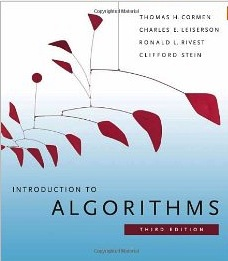
\includegraphics[width=.35\textwidth]{img/cormen.jpg}
    \\
    Introduction to Algorithms. Thomas H. Cormen, Charles E. Leiserson, Ronald L. Rivest. MIT Press, 1990 (disponível em português, em edições mais recentes).
  \end{tabular}
  \selectlanguage{brazil}

\end{frame}

\section{Problemas computacionais}

\begin{frame}
  \frametitle{Definição (problema computacional)}

  Um \emph{problema computacional\/} define como devem ser relacionados dados de
  entrada com dados de saída.

  \begin{block}{Exemplo}
    O problema da \emph{ordenação} pode der definido da seguinte maneira:
    \begin{quote}
      Seja $A$ um conjunto munido de uma relação de ordem total $\prec$.

      O problema da ordenação consiste em, dado uma sequência $a$ de $n$ valores
      $a_1, a_2, \ldots a_n$ de $A$, encontrar $a' = a'_1, a'_2, \ldots a'_n$ tal
      que
      \begin{itemize}
      \item $a'$ é uma permutação de $a$ e
      \item $a'_i \preceq a'_{i+1}$, para $1 \le i < n$.
      \end{itemize}
      Dados de entrada: $a$. Dados de saída: $a'$.
    \end{quote}
    \end{block}
\end{frame}

\begin{frame}
  \frametitle{Definição (instância de um problema computacional)}

  A \emph{instância} de um problema computacional é um caso particular de dados
  de entrada para um problema computacional.

  \begin{block}{Exemplo}
    Ordenar a seguinte sequência de inteiros usando a relação de ordem total $<$:
    \[
    3123, 214, 1011, 1125, 215, 10981, 42, 44648.
    \]
    \end{block}
\end{frame}

\begin{frame}
  \frametitle{Observações}

  \begin{itemize}
    \item Utilizamos várias noções matemáticas para definir o problema;
    \item Desvantagem: é um vocabulário específico.
    \item Vantagem: permite expressar-se de forma geral e precisa.
    \end{itemize}
\end{frame}

\begin{frame}
  \frametitle{Prática}

  Considere o seguinte enunciado (Manber 1989, ex~1.1):

  \selectlanguage{british}
  \begin{quote}
    Write down the numbers 1 to 100 each on a separate card. Shuffle the cards
    and rearrange them in order again.
  \end{quote}
  \selectlanguage{brazil}
  
  Qual(is) problema(s) computacional(is) está(ão) envolvidos nesta tarefa? 

  Expressar a resposta de duas maneiras:
  \begin{description}
  \item[informalmente:] em português somente;
  \item[formalmente:] em português e usando conceitos matemáticos.
  \end{description}
  
\end{frame}

\begin{frame}
  \frametitle{Prática}

  Considere o seguinte enunciado (Manber 1989, ex~1.2):

  \selectlanguage{british}
  \begin{quote}
    Write down the following 100 numbers each on a separate card. Shuffle the cards
    and rearrange them in order again.
    \[
    32918, 21192 , 11923 , 4233 , 88231 \cdots 11329 , 2253.
    \]
  \end{quote}
  \selectlanguage{brazil}
  
  Qual(is) problema(s) computacional(is) está(ão) envolvidos nesta tarefa? 

  Expressar a resposta de duas maneiras:
  \begin{description}
  \item[informalmente:] em português somente;
  \item[formalmente:] em português e usando conceitos matemáticos.
  \end{description}
  
\end{frame}

\begin{frame}
  \frametitle{Prática}

  Considere o seguinte enunciado (Manber 1989~1.3):

  \selectlanguage{british}
  \begin{quote}
    Consider the following list of numbers. Your job is to erase as few of those numbers as 
    possible such that the remaining numbers appear in increasing order. 
    \[
    \begin{array}{l}
    9, 44, 32, 12, 7, 42, 34, 92, 35, 37, 41, 8, 20, 27, 83, 64, 61, \\
    28, 39, 93, 29, 17, 13, 14, 55, 21, 66, 72, 23, 73, 99, 1, 2, 88, \\
    77, 4, 65, 83, 84, 62, 5, 11, 74, 68, 76, 78, 67, 75, 69, 70, 22, \\
    71, 24, 25, 26
    \end{array}
    \]
  \end{quote}
  \selectlanguage{brazil}

  
  Qual(is) problema(s) computacional(is) está(ão) envolvidos nesta tarefa? 

  Expressar a resposta de duas maneiras:
  \begin{description}
  \item[informalmente:] em português somente;
  \item[formalmente:] em português e usando conceitos matemáticos.
  \end{description}
  
\end{frame}

\begin{frame}
  \frametitle{Algoritmos: introdução}

  \selectlanguage{british}
  \begin{quotation}
    ``Science is what we understand well enough to explain to a computer; art is
    everything else.''

    --- Donald E. Knuth, Things a Computer Scientist Rarely Talks About.
  \end{quotation}
  \selectlanguage{brazil}

  Esta frase do cientista Knuth pode ser usada par ilustrar tanto o
  que ciência é quanto o que significa ``explicar coisas para um
  computador''.

  E explicar coisas para um computador é justamente o propósito de um 
  \emph{algoritmo}.

\end{frame}

\begin{frame}
  \frametitle{Algoritmos: introdução}

  \begin{quote}
  Um algoritmo é uma explicação passo a passo de como um computador deve
  resolver um problema computacional.
  \begin{enumerate}
  \item<1> ler uma instância do problema;
  \item<1-3> calcular o resultado esperado para esta instância;
  \item<1> fornecer este resultado.
  \end{enumerate}
  \end{quote}
  \pause
  \pause
  \begin{description}
  \item[explicação:] em qual linguagem deve-se realizada?
  \item[passo a passo:] quais são os passos básicos que um computador
    pode executar?
  \end{description}
  Esta explicação depois é traduzida \emph{manualmente} em uma linguagem
  de programação de computadores.

\end{frame}

\begin{frame}

  \frametitle{Algoritmos: o modelo computacional}

  \begin{itemize}
  \item \textit{Random Access Machine}: 
    \begin{itemize}
      \item processador
      \item memória
      \item (dispositivo de entrada)
      \item (dispositivo de saída)
    \end{itemize}
  \item algoritmo/programa: lista de instruções;
  \item o processador executa uma instrução por vez;
  \item fluxo: instruções são executadas em sequência;
  \item mas o fluxo pode ser desviado para uma instrução qualquer
    condicionalmente ou incondicionalmente.
  \end{itemize}
\end{frame}

\begin{frame}

  \frametitle{Algoritmos: precisão mas não padronização}

  \begin{itemize}
  \item Quase cada livro e cada autor possui uma notação algorítmica diferente!

  \item O algoritmo é traduzido \emph{manualmente} em uma linguagem de
    programação de computadores.

  \item A notação algorítmica é intepretada por um ser humano.

  \item A linguagem de programção é interpretada por uma máquina.

  \item A notação algorítmica deve ao mesmo tempo não ter ambigüidade e pode ser
    livre das amarras impostas pelas linguagens de programação.

  \item As notações algorítmicas se equivalem essencialmente.

  \end{itemize}

\end{frame}

\begin{frame}

  \frametitle{Algoritmos: os padrões estruturais}

  \begin{itemize}
  \item identificar dados a serem manipulados: var
  \item estruturar dados: array, pointer, record, enum
  \item execução condicional de um bloco de comandos: \If 
  \item repetição condicional de um bloco de comandos: \While
    \begin{itemize}
    \item \For, \To, \Downto
    \end{itemize}
  \item alterar um dado: $\gets$
  \item agrupar blocos de comandos
  \item agrupar e nomear um bloco de comandos (sub-rotina)
  \item redirecionamento: \Goto
  \item indentação é usada para identificar os blocos.
  \end{itemize}
\end{frame}

\begin{frame}

  \frametitle{Algoritmo: ordenação por inserção}

(Cormen et al. 1990)

\begin{codebox}
\Procname{$\proc{Insertion-Sort}(A)$}
\li \For $j \gets 2$ \To $\id{length}[A]$
\li     \Do
$\id{key} \gets A[j]$
\li
\Comment Insert $A[j]$ into the sorted sequence
    $A[1 \twodots j-1]$.
\li $i \gets j-1$
\li \While $i > 0$ and $A[i] > \id{key}$
\li    \Do
        $A[i+1] \gets A[i]$
\li     $i \gets i-1$
    \End
\li $A[i+1] \gets \id{key}$
\End
\end{codebox}  
\Comment indica que o resto da linha é um \emph{comentário}.
\end{frame}

\begin{frame}

  \frametitle{Ordenação por inserção: exemplo}

  \[
  A = \begin{array}{cccccc}
8 & 2 & 4 & 9 & 3 & 6
\end{array}
\]


\begin{codebox}
\Procname{$\proc{Insertion-Sort}(A)$}
\li \For $j \gets 2$ \To $\id{length}[A]$
\li     \Do
$\id{key} \gets A[j]$
\li
\Comment Insert $A[j]$ into the sorted sequence
    $A[1 \twodots j-1]$.
\li $i \gets j-1$
\li \While $i > 0$ and $A[i] > \id{key}$
\li    \Do
        $A[i+1] \gets A[i]$
\li     $i \gets i-1$
    \End
\li $A[i+1] \gets \id{key}$
\End
\end{codebox}  

\end{frame}

\begin{frame}

  \frametitle{Ordenação por inserção: exercício}

\begin{codebox}
\Procname{$\proc{Insertion-Sort}(A)$}
\li \For $j \gets 2$ \To $\id{length}[A]$
\li     \Do
$\id{key} \gets A[j]$
\li
\Comment Insert $A[j]$ into the sorted sequence
    $A[1 \twodots j-1]$.
\li $i \gets j-1$
\li \While $i > 0$ and $A[i] > \id{key}$
\li    \Do
        $A[i+1] \gets A[i]$
\li     $i \gets i-1$
    \End
\li $A[i+1] \gets \id{key}$
\End
\end{codebox}  

\begin{enumerate}
\item Aplique o algoritmo para $A = \langle 31, 41, 59, 26, 41, 58 \rangle$.
\item Reescreva o procedimento \proc{Insertion-Sort} para ordenar em ordem
  decrescente.
\end{enumerate}
(Cormen et al. 1990)

\end{frame}

\begin{frame}

  \frametitle{Algoritmos: exercício}

Considere o problema da \emph{busca}:

\begin{description}
\item[entrada] Uma sequência de $n$ valores $A = \langle a_1, a_2, \ldots a_n \rangle$
e um valor $v$.
\item[resultado] Um índice $i$ tal que $a_i = v$ ou um valor especial \const{nil} se $v$ não pertence a $A$.
\end{description}

Escreva o algoritmo da \emph{busca linear} que resolve este problema.

(Cormen et al. 1990)

\end{frame}

\section{Análise de algoritmos}

\begin{frame}

  \frametitle{Algoritmo: análise}

  O algoritmo calcule o resultado esperado? o algoritmo faz uso eficiente dos
  recursos computacionais?
  \begin{description}
  \item[correção] O algoritmo é correto? 
  \item[complexidade] Quais recursos o computador usará para executar este
    algoritmo?
    \begin{itemize}
    \item tempo
    \item memória
    \end{itemize}
  \end{description}

\end{frame}

\begin{frame}

  \frametitle{Correção de algoritmos}

  Um algoritmo para um determinado problema computacional $P$ é \emph{correto}
  quando cada vez que é aplicado a uma instância do problema:
  \pause
  \begin{itemize}
    \item ele calcula o resultado em um número finito de passos;
    \item o resultado calculado é o mesmo que especificado na descrição do
      problema $P$.
  \end{itemize}

\end{frame}

\begin{frame}

  \frametitle{Correção de algoritmos}

  É mais fácil mostrar que um algoritmo \emph{não} é correto!
  \pause

  \begin{block}{Receita para provar que um algoritmo é incorreto.}
  Basta encontrar uma instância do problema tratado tal que:
  \begin{itemize}
    \item o algoritmo executa-se infinitamente, ou
    \item o algoritmo termina em um número finito de passos e o resultado
      calculado não é o mesmo que especificado na descrição do problema $P$.
  \end{itemize}
  \end{block}

\end{frame}

\begin{frame}

  \frametitle{Exercício: Mostre que o algoritmo é incorreto}

\begin{codebox}
\Procname{$\proc{Linear-Search}(A, v)$}
\li $j \gets 1$
\li \While $A[j] \neq v$
\li \Do
      $j \gets j+1$
    \End
\li \Return $j$
\end{codebox}  

\end{frame}

\begin{frame}
  \frametitle{Exercício: Mostre que o algoritmo é incorreto}

\begin{codebox}
\Procname{$\proc{Linear-Search}(A, v)$}
\li $j \gets 1$
\li \While $A[j] \neq v$ and $j < \id{length}[A]$
\li \Do
      $j \gets j+1$
    \End
\li \Return $j$
\end{codebox}  

\end{frame}

\begin{frame}

\frametitle{Exercício: Mostre que o algoritmo é incorreto}

\begin{codebox}
\Procname{$\proc{Linear-Search}(A, v)$}
\li $j \gets 1$
\li \While $A[j] \neq v$ and $j \le \id{length}[A]$
\li \Do
      $j \gets j+1$
    \End
\li \Return $j$
\end{codebox}  

\end{frame}

\begin{frame}

\frametitle{Versão final}

\begin{codebox}
\Procname{$\proc{Linear-Search}(A, v)$}
\li $j \gets 1$
\li \While $A[j] \neq v$ and $j \le \id{length}[A]$
\li \Do
      $j \gets j+1$
    \End
\li \If $j \le \id{length}[A]$
\li \Then
      \Return $j$
\li \Else
      \Return \const{nil}
    \End
\end{codebox}  

\pause

O algoritmo $A$ é correto se e somente se 
\begin{itemize}
\item ele não é incorreto. \pause
\item $\neg \exists$ instância $i$ do problema t.q. $A(i)$ não termina ou tem um resultado errado. \pause
\item $\forall$ instancia $i$ do problema, $A(i)$ termina com resultado certo.
\end{itemize}

\end{frame}

\begin{frame}

\frametitle{Exercício}

\begin{itemize}

  \item Supondo que não seja autorizado avaliar $A[j]$ quando $j \le
    0$ ou $j > \id{length}[A]$, o algoritmo continua correto?

  \item Se não for correto, como corrigir?

  \item O que acontece quando $A$ é uma sequência de zero elementos? Está em
conformidade com a especificação?

\end{itemize}

\end{frame}

\begin{frame}

\frametitle{``Mostre que o algoritmo é correto''. Como responder?}

\begin{itemize}
\item A definição de algoritmo correto não é operacional: não é possível
enumerar todas as instâncias e verificar que o algoritmo termina com o resultado certo.
\end{itemize}

\begin{quote}
Program testing can be used to show bugs, but never their absence!

--- \href{http://en.wikipedia.org/wiki/Edsger_W._Dijkstra}{Edsger Dijkstra} (1930--2002).
\end{quote}

\begin{itemize}
\item Mostrar que um algoritmo é correto requer utilizar técnicas de prova mais
  elaboradas que enumeração e cálculo.
\end{itemize}

\pause

\begin{center}
$\Rightarrow$ \emph{Lógica de Hoare}
\end{center}

\end{frame}

\begin{frame}

  \frametitle{Complexidade de um algoritmo}

  \begin{itemize}
    \item Um mesmo problema pode ser resolvido de várias maneiras diferentes.
    \item Como escolher entre diversos algoritmos?
    \item Estimar \emph{o tempo de execução\/} de cada algoritmo.

      \emph{Complexidade\/} do algoritmo
  \end{itemize}

\end{frame}

\begin{frame}
\frametitle{Complexidade de algoritmo}

\begin{itemize}
\item Como quantificar a complexidade (temporal) de um algoritmo?
\item Conta como?

\pause
\begin{itemize}
  \item Quantas vezes cada instrução é executada.
\end{itemize}

\item Depende de quê?

\pause
\begin{itemize}
\item Do \emph{tamanho\/} da entrada.
\item Do \emph{valor\/} da entrada.
\end{itemize}
\end{itemize}

\end{frame}

\end{document}
